\documentclass[10pt,journal,compsoc]{IEEEtran}

\usepackage{amsmath,amssymb,amsfonts}
\usepackage{graphicx}
\usepackage{tikz}
\usepackage{booktabs}
\usepackage{hyperref}
\usepackage{cite}
\usepackage{microtype}
\usepackage{xcolor}

\usetikzlibrary{shapes,arrows,positioning,calc,decorations.pathmorphing,patterns}

\hypersetup{
    colorlinks=true,
    linkcolor=blue!70!black,
    citecolor=blue!70!black,
    urlcolor=blue!70!black
}

\begin{document}

\title{Design, Multi-Tier Microwave Modeling, and Physical Layout Synthesis of a 7-Qubit Superconducting Transmon Processor}

\author{Atharve~Dahima
\thanks{A. Dahima is with the Quantum Hardware and Cryogenic Electronics Research Group. Inquiries: \texttt{atharveeee@gmail.com}.}}

\markboth{IEEE Transactions on Applied Superconductivity / Quantum Engineering, Preprint 2026}%
{Dahima: Design and Layout Synthesis of a 7-Qubit Transmon Processor}

\maketitle

\begin{abstract}
Superconducting quantum processors operating in the circuit quantum electrodynamics (cQED) regime represent one of the most viable architectures for scalable, fault-tolerant quantum computation. This treatise presents the end-to-end design, multi-tier microwave modeling, and lithographic layout synthesis of a planar 7-qubit superconducting transmon processor based on the landmark IBM hexagonal-radial lattice. We develop an integrated design methodology comprising: (1) First-principles Hamiltonian formulation and non-linear Josephson potential derivation; (2) Dilution refrigeration thermal engineering and cryogenic microwave attenuation profiling; (3) Tier-1 lumped-element equivalent network synthesis in Ansys Circuit to verify loaded quality factors and transmission notches ($S_{21}$); (4) Tier-2 planar thin-film layout synthesis in Qiskit Metal targeting 50-$\Omega$ coplanar waveguide (CPW) transmission lines; and (5) Tier-3 full-wave 3D Finite Element Method (FEM) eigenmode simulation and Energy Participation Ratio (EPR) quantization in Ansys HFSS. An exhaustive mathematical lexicon of cQED terminology is provided to serve as a standardized theoretical reference for superconducting device engineering.
\end{abstract}

\begin{IEEEkeywords}
Circuit QED, Transmon Qubit, Josephson Junction, Coplanar Waveguide, Ansys HFSS, Qiskit Metal, Energy Participation Ratio (EPR), S-Parameters.
\end{IEEEkeywords}

\section{Introduction and Quantum Hardware Modalities}
\IEEEPARstart{A}{mong} competing quantum physical implementations---including trapped atomic ions, neutral Rydberg atoms, photonic circuits, and semiconductor quantum dots---superconducting circuits uniquely bridge quantum mechanics and macroscopic microwave engineering. Superconducting qubits leverage Cooper-pair condensates in lithographically patterned thin-film metals (e.g., Niobium and Aluminum), operating at microwave frequencies ($4\text{--}8\text{ GHz}$). 

Unlike trapped ions that require high-vacuum laser enclosures or photonic circuits demanding non-deterministic single-photon gates, superconducting artificial atoms are fabricated using mature semiconductor planar lithography. Microwave pulses routed through $50\,\Omega$ coaxial transmission lines manipulate the quantum state via electric dipole coupling ($\hat{d} \cdot \vec{E}$), enabling nanosecond-scale gate execution.

\begin{figure}[!t]
\centering
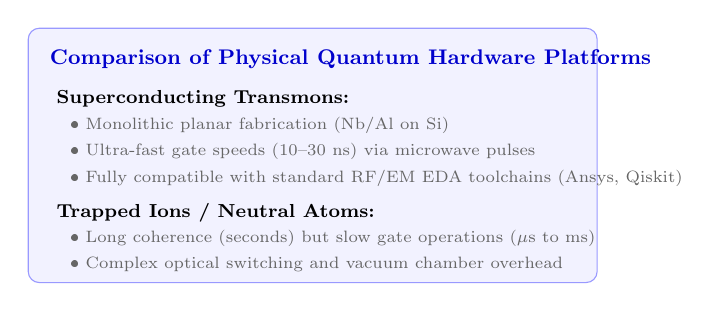
\begin{tikzpicture}[scale=0.85, every node/.style={transform shape}]
    \draw[fill=blue!5, draw=blue!40, rounded corners=4pt] (0,0) rectangle (8.5, 3.8);
    \node[anchor=north west, font=\bfseries\small, text=blue!80!black] at (0.2, 3.6) {Comparison of Physical Quantum Hardware Platforms};
    
    \node[anchor=north west, font=\footnotesize] at (0.3, 3.0) {\textbf{Superconducting Transmons:}};
    \node[anchor=north west, font=\scriptsize, text=gray!80!black] at (0.5, 2.6) {• Monolithic planar fabrication (Nb/Al on Si)};
    \node[anchor=north west, font=\scriptsize, text=gray!80!black] at (0.5, 2.2) {• Ultra-fast gate speeds (10--30 ns) via microwave pulses};
    \node[anchor=north west, font=\scriptsize, text=gray!80!black] at (0.5, 1.8) {• Fully compatible with standard RF/EM EDA toolchains (Ansys, Qiskit)};
    
    \node[anchor=north west, font=\footnotesize] at (0.3, 1.3) {\textbf{Trapped Ions / Neutral Atoms:}};
    \node[anchor=north west, font=\scriptsize, text=gray!80!black] at (0.5, 0.9) {• Long coherence (seconds) but slow gate operations ($\mu$s to ms)};
    \node[anchor=north west, font=\scriptsize, text=gray!80!black] at (0.5, 0.5) {• Complex optical switching and vacuum chamber overhead};
\end{tikzpicture}
\caption{Taxonomy of quantum modalities, highlighting the engineering scalability and high clock frequencies of superconducting circuit QED.}
\label{fig:modalities}
\end{figure}

\section{Cryogenic Hardware Infrastructure and Thermal Isolation}
Superconducting quantum processors require operation at absolute temperatures $T \approx 10\text{--}15\text{ mK}$, achieved through closed-cycle helium dilution refrigeration ($^3\text{He}/^4\text{He}$ dilution). At room temperature ($300\text{ K}$), thermal energy $k_B T \approx 25.8\text{ meV}$ swamps the single-photon microwave energy:
\begin{equation}
\hbar \omega_{01} \approx h \times 5.0\text{ GHz} \approx 20.7\,\mu\text{eV}
\end{equation}
Thermal equilibrium at $10\text{ mK}$ yields $k_B T \approx 0.86\,\mu\text{eV}$, ensuring the Boltzmann occupation probability of the first excited state $|1\rangle$ is negligible:
\begin{equation}
P_1 = \exp\left(-\frac{\hbar \omega_{01}}{k_B T}\right) \approx \exp\left(-\frac{20.7}{0.86}\right) \approx 3.9 \times 10^{-11}
\end{equation}
thereby freezing the circuit into its quantum ground state $|0\rangle$.

\begin{figure}[!b]
\centering
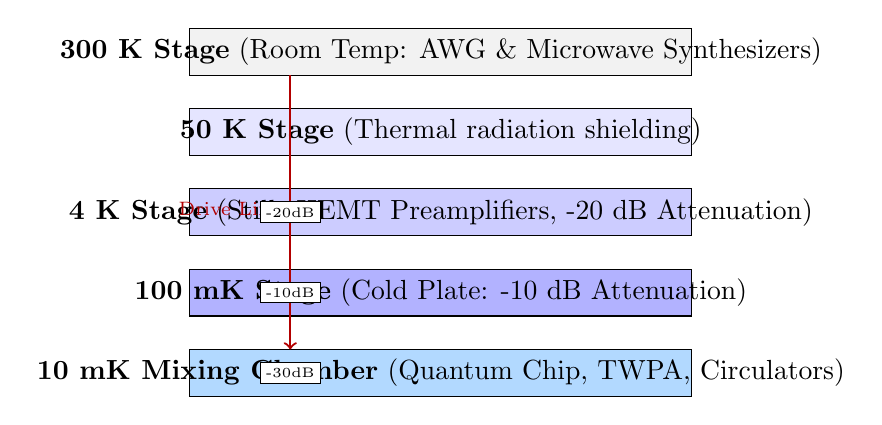
\begin{tikzpicture}[scale=0.85]
    \draw[fill=gray!10, draw=black] (0,4.5) rectangle (7.5, 5.2);
    \node at (3.75, 4.85) {\textbf{300 K Stage} (Room Temp: AWG \& Microwave Synthesizers)};
    
    \draw[fill=blue!10, draw=black] (0,3.3) rectangle (7.5, 4.0);
    \node at (3.75, 3.65) {\textbf{50 K Stage} (Thermal radiation shielding)};
    
    \draw[fill=blue!20, draw=black] (0,2.1) rectangle (7.5, 2.8);
    \node at (3.75, 2.45) {\textbf{4 K Stage} (Still: HEMT Preamplifiers, -20 dB Attenuation)};
    
    \draw[fill=blue!30, draw=black] (0,0.9) rectangle (7.5, 1.6);
    \node at (3.75, 1.25) {\textbf{100 mK Stage} (Cold Plate: -10 dB Attenuation)};
    
    \draw[fill=blue!50!cyan!30, draw=black] (0,-0.3) rectangle (7.5, 0.4);
    \node at (3.75, 0.05) {\textbf{10 mK Mixing Chamber} (Quantum Chip, TWPA, Circulators)};
    
    \draw[thick, red!70!black, ->] (1.5, 4.5) -- (1.5, 4.0) -- (1.5, 2.8) -- (1.5, 1.6) -- (1.5, 0.4);
    \node[left, font=\scriptsize, text=red!70!black] at (1.5, 2.5) {Drive Line};
    
    \node[draw, fill=white, inner sep=2pt, font=\tiny] at (1.5, 2.45) {-20dB};
    \node[draw, fill=white, inner sep=2pt, font=\tiny] at (1.5, 1.25) {-10dB};
    \node[draw, fill=white, inner sep=2pt, font=\tiny] at (1.5, 0.05) {-30dB};
\end{tikzpicture}
\caption{Thermal stratification of a dilution refrigerator. Attenuators thermalize blackbody microwave photons descending from room temperature down to 10 mK.}
\label{fig:fridge}
\end{figure}

\section{Superconducting Transmon Physics and Hamiltonian Formulation}

\subsection{Harmonic Oscillator Leakage Catastrophe}
A linear LC tank resonator consisting of an inductor $L$ and capacitor $C$ exhibits a quadratic potential $U(\Phi) = \Phi^2 / 2L$. Solving the Schr\"odinger equation yields strictly equidistant eigenenergies:
\begin{equation}
E_n = \hbar \omega_0 \left(n + \frac{1}{2}\right), \quad \omega_0 = \frac{1}{\sqrt{LC}}
\end{equation}
Because transition frequencies are identical ($\omega_{01} = \omega_{12} = \omega_{23}$), an applied microwave drive at frequency $\omega_{01}$ cannot isolate a two-level qubit; it induces catastrophic multi-photon ladder climbing into higher excited states $|n \ge 2\rangle$.

\subsection{Josephson Non-Linearity and the Duffing Oscillator}
To achieve spectral anharmonicity, the linear inductor is replaced with a sub-micron Al/$\text{Al}_2\text{O}_3$/Al Josephson tunnel junction. The gauge-invariant phase difference across the junction $\hat{\phi} = 2\pi \Phi / \Phi_0$ governs the dissipationless supercurrent:
\begin{equation}
I(t) = I_c \sin\hat{\phi}, \quad V(t) = \frac{\Phi_0}{2\pi} \frac{d\hat{\phi}}{dt}
\end{equation}
where $\Phi_0 = h/2e$ is the superconducting magnetic flux quantum and $I_c$ is the junction critical current. The inductive energy stored in the junction is:
\begin{equation}
U(\hat{\phi}) = -E_J \cos\hat{\phi} \approx -E_J \left( 1 - \frac{\hat{\phi}^2}{2} + \frac{\hat{\phi}^4}{24} - \dots \right)
\end{equation}
The quadratic term provides linear inductance $L_{J0} = \Phi_0 / (2\pi I_c)$, while the negative quartic perturbation $-\frac{E_J}{24}\hat{\phi}^4$ compresses higher energy levels, introducing a non-zero Duffing anharmonicity $\alpha$:
\begin{equation}
\alpha = \omega_{12} - \omega_{01} \approx -E_C
\end{equation}
where $E_C = e^2 / (2C_\Sigma)$ is the single-electron charging energy.

\begin{figure}[!t]
\centering
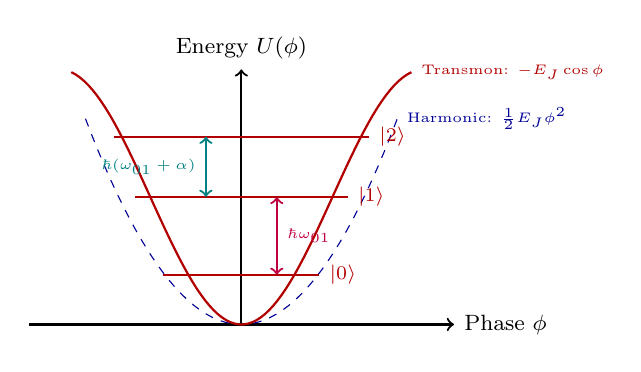
\begin{tikzpicture}[scale=0.9]
    \draw[->, thick] (-3,0) -- (3,0) node[right, font=\footnotesize] {Phase $\phi$};
    \draw[->, thick] (0,0) -- (0,3.6) node[above, font=\footnotesize] {Energy $U(\phi)$};
    
    \draw[dashed, blue!60!black, domain=-2.2:2.2, samples=50] plot (\x, {0.6*\x*\x}) node[right, font=\tiny] {Harmonic: $\frac{1}{2} E_J \phi^2$};
    \draw[thick, red!70!black, domain=-2.4:2.4, samples=80] plot (\x, {1.8*(1 - cos(\x*70))}) node[right, font=\tiny] {Transmon: $-E_J \cos\phi$};
    
    \draw[red!70!black, thick] (-1.1, 0.7) -- (1.1, 0.7) node[right, font=\scriptsize] {$|0\rangle$};
    \draw[red!70!black, thick] (-1.5, 1.8) -- (1.5, 1.8) node[right, font=\scriptsize] {$|1\rangle$};
    \draw[red!70!black, thick] (-1.8, 2.65) -- (1.8, 2.65) node[right, font=\scriptsize] {$|2\rangle$};
    
    \draw[<->, purple, thick] (0.5, 0.7) -- (0.5, 1.8) node[midway, right, font=\tiny] {$\hbar\omega_{01}$};
    \draw[<->, teal, thick] (-0.5, 1.8) -- (-0.5, 2.65) node[midway, left, font=\tiny] {$\hbar(\omega_{01} + \alpha)$};
\end{tikzpicture}
\caption{Comparison of the parabolic potential (equidistant ladder) versus the cosinusoidal Josephson potential, demonstrating the negative anharmonic shift $\alpha = \omega_{12} - \omega_{01} \approx -E_C$.}
\label{fig:anharmonicity}
\end{figure}

\subsection{The Transmon Regime ($E_J / E_C \approx 50$)}
The Cooper-Pair Box Hamiltonian is given by:
\begin{equation}
\hat{H} = 4 E_C (\hat{n} - n_g)^2 - E_J \cos\hat{\phi}
\end{equation}
where $\hat{n} = -i \partial / \partial \phi$ is the Cooper-pair number operator and $n_g = Q_r / 2e$ is the dimensionless offset gate charge.

In the transmon limit ($E_J / E_C \gg 1$), charge dispersion $\epsilon_m$ decays exponentially:
\begin{equation}
\epsilon_m \approx (-1)^m E_C \frac{2^{4m+5}}{m!} \sqrt{\frac{2}{\pi}} \left(\frac{E_J}{2E_C}\right)^{\frac{m}{2} + \frac{3}{4}} \exp\left(-\sqrt{\frac{8E_J}{E_C}}\right)
\end{equation}
By shunting the junction with large coplanar capacitor pads to set $C_\Sigma \approx 70\text{ fF}$ and $E_J/E_C \approx 50$, charge dephasing is suppressed by orders of magnitude while preserving an anharmonicity of $|\alpha|/2\pi \approx 280\text{--}330\text{ MHz}$.

\section{Circuit QED and Readout Resonator Synthesis}

\subsection{Coplanar Waveguide (CPW) Conformal Mapping}
Transmission of microwave signals across the chip is accomplished using Coplanar Waveguides (CPW), consisting of a center conductor of width $W = 10\,\mu\text{m}$ separated by gaps $S = 6\,\mu\text{m}$ from continuous ground planes on high-resistivity silicon ($\epsilon_r = 11.45$).

\begin{figure}[!t]
\centering
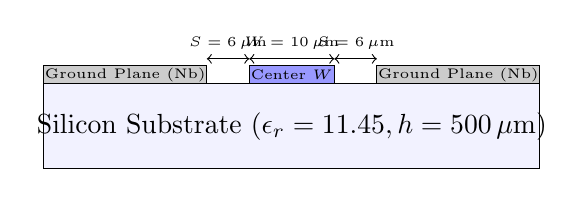
\begin{tikzpicture}[scale=0.9]
    \draw[fill=blue!5, draw=black] (-3.5, -1.2) rectangle (3.5, 0);
    \node at (0, -0.6) {Silicon Substrate ($\epsilon_r = 11.45, h = 500\,\mu\text{m}$)};
    
    \draw[fill=gray!40, draw=black] (-3.5, 0) rectangle (-1.2, 0.25);
    \draw[fill=gray!40, draw=black] (1.2, 0) rectangle (3.5, 0.25);
    \node at (-2.35, 0.12) {\tiny Ground Plane (Nb)};
    \node at (2.35, 0.12) {\tiny Ground Plane (Nb)};
    
    \draw[fill=blue!40, draw=black] (-0.6, 0) rectangle (0.6, 0.25);
    \node at (0, 0.12) {\tiny Center $W$};
    
    \draw[<->] (-1.2, 0.35) -- (-0.6, 0.35) node[midway, above, font=\tiny] {$S = 6\,\mu\text{m}$};
    \draw[<->] (-0.6, 0.35) -- (0.6, 0.35) node[midway, above, font=\tiny] {$W = 10\,\mu\text{m}$};
    \draw[<->] (0.6, 0.35) -- (1.2, 0.35) node[midway, above, font=\tiny] {$S = 6\,\mu\text{m}$};
\end{tikzpicture}
\caption{Cross-sectional geometry of a Coplanar Waveguide (CPW) designed for $50\,\Omega$ characteristic impedance on high-resistivity silicon.}
\label{fig:cpw}
\end{figure}

The effective dielectric constant $\epsilon_{\text{eff}}$ and characteristic impedance $Z_0$ are derived via complete elliptic integrals of the first kind $K(k)$:
\begin{equation}
\epsilon_{\text{eff}} \approx \frac{\epsilon_r + 1}{2} = \frac{11.45 + 1}{2} \approx 6.225
\end{equation}
\begin{equation}
Z_0 = \frac{30\pi}{\sqrt{\epsilon_{\text{eff}}}} \frac{K(k')}{K(k)} = 50.0\,\Omega, \quad k = \frac{W}{W + 2S} = \frac{10}{22}
\end{equation}

\subsection{Quarter-Wavelength ($\lambda/4$) Dispersive Resonators}
A $\lambda/4$ resonator is shorted to ground at one end (current antinode) and capacitively coupled at the open end (voltage antinode). The physical length $l$ required to achieve $f_r \approx 7.0\text{ GHz}$ is:
\begin{equation}
l = \frac{v_{\text{ph}}}{4 f_r} = \frac{c}{4 f_r \sqrt{\epsilon_{\text{eff}}}} = \frac{3 \times 10^8}{4 \times 7.0\times 10^9 \times \sqrt{6.225}} \approx 4.29\text{ mm}
\end{equation}
The meandered geometry minimizes on-chip real estate while maintaining sufficient spatial separation ($> 300\,\mu\text{m}$) to prevent slotline cross-coupling.

\subsection{Dispersive Readout and Purcell Filtering}
Operating in the dispersive limit ($|\Delta| = |\omega_{01} - \omega_r| \gg g$), the dressed Hamiltonian becomes:
\begin{equation}
\hat{H}_{\text{disp}} \approx \hbar \left(\omega_r + \chi \hat{\sigma}_z\right) \hat{a}^\dagger \hat{a} + \frac{1}{2} \hbar \tilde{\omega}_{01} \hat{\sigma}_z
\end{equation}
The state-dependent dispersive shift $\chi$ pulls the resonator frequency by $\pm \chi$:
\begin{equation}
\chi \approx \frac{g^2}{\Delta} \frac{\alpha}{\Delta + \alpha}
\end{equation}
To prevent spontaneous Purcell relaxation of the qubit through the readout feedline ($\gamma_\kappa = \kappa (g/\Delta)^2$), a loaded quality factor $Q_L \approx 7,000$ is established via input coupling capacitor $C_{\text{in}} \approx 2.0\text{ fF}$.

\section{7-Qubit Processor Topology and Frequency Allocation}
To suppress parasitic swap interactions during idle states, a staggered frequency plan is established across the radial 7-qubit architecture:

\begin{figure}[!t]
\centering
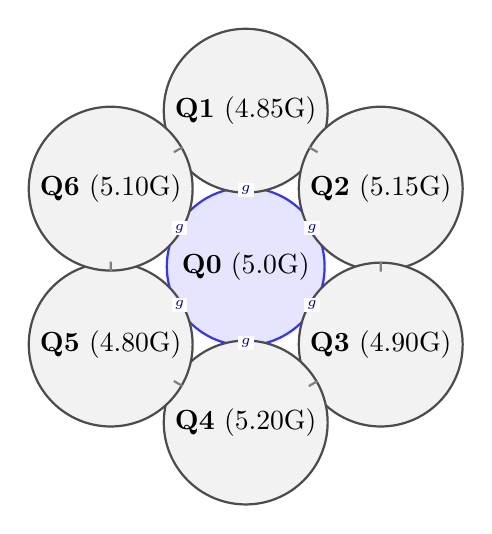
\begin{tikzpicture}[scale=0.9]
    \node[circle, draw=blue!80, fill=blue!10, thick, inner sep=4pt] (Q0) at (0,0) {\textbf{Q0} (5.0G)};
    
    \foreach \ang/\idx/\fq in {90/1/4.85G, 30/2/5.15G, 330/3/4.90G, 270/4/5.20G, 210/5/4.80G, 150/6/5.10G} {
        \node[circle, draw=black!70, fill=gray!10, thick, inner sep=3pt] (Q\idx) at (\ang:2.2) {\textbf{Q\idx} (\fq)};
        \draw[thick, dashed, blue!60!black] (Q0) -- (Q\idx) node[midway, fill=white, inner sep=1pt, font=\tiny] {$g$};
    }
    \draw[thick, gray] (Q1) -- (Q2) -- (Q3) -- (Q4) -- (Q5) -- (Q6) -- (Q1);
\end{tikzpicture}
\caption{Landmark IBM 7-qubit radial lattice. Central tunable transmon $Q_0$ interacts with six perimeter fixed-frequency qubits ($Q_1$--$Q_6$) with staggered frequencies to prevent spectral collision.}
\label{fig:lattice}
\end{figure}

\begin{table}[!h]
\centering
\caption{7-Qubit Frequency and Coupling Allocation}
\label{tab:allocation}
\begin{tabular}{lcccc}
\toprule
\textbf{Qubit} & $f_{01}\text{ (GHz)}$ & $\alpha\text{ (MHz)}$ & $f_r\text{ (GHz)}$ & Coupling Target \\
\midrule
$Q_0\text{ (Center)}$ & $5.00$ & $-300$ & $7.00$ & Bus to $Q_1$--$Q_6$ \\
$Q_1$ & $4.85$ & $-290$ & $6.85$ & $Q_0, Q_2, Q_6$ \\
$Q_2$ & $5.15$ & $-310$ & $7.15$ & $Q_0, Q_1, Q_3$ \\
$Q_3$ & $4.90$ & $-295$ & $6.90$ & $Q_0, Q_2, Q_4$ \\
$Q_4$ & $5.20$ & $-315$ & $7.20$ & $Q_0, Q_3, Q_5$ \\
$Q_5$ & $4.80$ & $-285$ & $6.80$ & $Q_0, Q_4, Q_6$ \\
$Q_6$ & $5.10$ & $-305$ & $7.10$ & $Q_0, Q_5, Q_1$ \\
\bottomrule
\end{tabular}
\end{table}

\section{Cleanroom Fabrication and Shadow Evaporation}
Planar device realization follows a multi-step lithography process:
\begin{enumerate}
    \item \textbf{Base Metallization:} A $200\text{ nm}$ continuous Niobium film is sputtered onto high-resistivity ($>10\text{ k}\Omega\cdot\text{cm}$) float-zone Silicon. Optical lithography and Reactive Ion Etching (RIE) pattern the CPW ground planes and large transmon pads.
    \item \textbf{EBL Patterning:} Bilayer resist (MMA/PMMA) is spun and exposed via Electron Beam Lithography to define the suspended Dolan resist bridge.
    \item \textbf{Dolan Bridge Shadow Evaporation:} The sample is loaded into an ultra-high vacuum e-beam evaporator. Aluminum is evaporated at angle $+\theta$, followed by controlled static oxidation ($P_{\text{O}_2} \approx 1\text{ Torr}, t \approx 10\text{ min}$) to form the $\text{Al}_2\text{O}_3$ barrier, concluded by a second deposition at angle $-\theta$.
\end{enumerate}

\begin{figure}[!h]
\centering
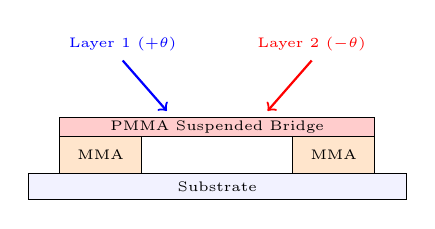
\begin{tikzpicture}[scale=0.8]
    \draw[fill=blue!5, draw=black] (-3,0) rectangle (3, 0.4);
    \node at (0, 0.2) {\tiny Substrate};
    
    \draw[fill=orange!20, draw=black] (-2.5, 0.4) rectangle (-1.2, 1.0);
    \draw[fill=orange!20, draw=black] (1.2, 0.4) rectangle (2.5, 1.0);
    \node at (-1.85, 0.7) {\tiny MMA};
    \node at (1.85, 0.7) {\tiny MMA};
    
    \draw[fill=red!20, draw=black] (-2.5, 1.0) rectangle (2.5, 1.3);
    \node at (0, 1.15) {\tiny PMMA Suspended Bridge};
    
    \draw[->, thick, blue] (-1.5, 2.2) -- (-0.8, 1.4);
    \draw[->, thick, red] (1.5, 2.2) -- (0.8, 1.4);
    \node[above, font=\tiny, text=blue] at (-1.5, 2.2) {Layer 1 ($+\theta$)};
    \node[above, font=\tiny, text=red] at (1.5, 2.2) {Layer 2 ($-\theta$)};
\end{tikzpicture}
\caption{Dolan bridge shadow evaporation. Bilayer resist profile provides undercut, enabling angled double-evaporation of Al/$\text{Al}_2\text{O}_3$/Al junctions.}
\label{fig:dolan}
\end{figure}

\section{Tier-1: Lumped-Element Circuit Synthesis}
Using Ansys Electronics Desktop (Nexxim Circuit), the classical equivalent representation is simulated prior to 3D geometry layout.

\begin{figure}[!h]
\centering
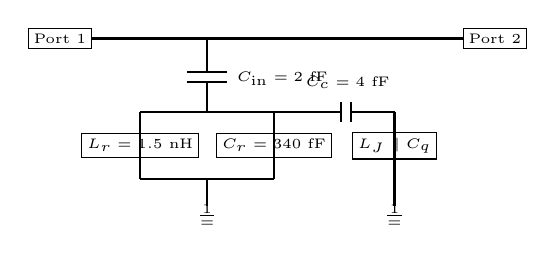
\begin{tikzpicture}[scale=0.85]
    \draw[thick] (0, 2.5) -- (6.5, 2.5);
    \node[draw, fill=white, inner sep=2pt, font=\tiny] at (0, 2.5) {Port 1};
    \node[draw, fill=white, inner sep=2pt, font=\tiny] at (6.5, 2.5) {Port 2};
    
    \draw[thick] (2.2, 2.5) -- (2.2, 2.0);
    \draw[thick] (1.9, 2.0) -- (2.5, 2.0);
    \draw[thick] (1.9, 1.85) -- (2.5, 1.85);
    \draw[thick] (2.2, 1.85) -- (2.2, 1.4);
    \node[right, font=\tiny] at (2.5, 1.9) {$C_{\text{in}} = 2\text{ fF}$};
    
    \draw[thick] (1.2, 1.4) -- (3.2, 1.4);
    \draw[thick] (1.2, 1.4) -- (1.2, 0.4);
    \draw[thick] (3.2, 1.4) -- (3.2, 0.4);
    \node[draw, inner sep=2pt, font=\tiny] at (1.2, 0.9) {$L_r = 1.5\text{ nH}$};
    \node[draw, inner sep=2pt, font=\tiny] at (3.2, 0.9) {$C_r = 340\text{ fF}$};
    \draw[thick] (1.2, 0.4) -- (3.2, 0.4);
    \draw[thick] (2.2, 0.4) -- (2.2, 0.0);
    \node at (2.2, -0.15) {\tiny $\frac{1}{=}$};
    
    \draw[thick] (3.2, 1.4) -- (4.2, 1.4);
    \draw[thick] (4.2, 1.55) -- (4.2, 1.25);
    \draw[thick] (4.35, 1.55) -- (4.35, 1.25);
    \draw[thick] (4.35, 1.4) -- (5.0, 1.4);
    \node[above, font=\tiny] at (4.3, 1.6) {$C_c = 4\text{ fF}$};
    
    \draw[thick] (5.0, 1.4) -- (5.0, 0.4);
    \node[draw, inner sep=2pt, font=\tiny] at (5.0, 0.9) {$L_J \parallel C_q$};
    \draw[thick] (5.0, 0.4) -- (5.0, 0.0);
    \node at (5.0, -0.15) {\tiny $\frac{1}{=}$};
\end{tikzpicture}
\caption{Lumped-element equivalent circuit implemented in Ansys Circuit to verify the $S_{21}$ transmission notch at $f_r \approx 7.04\text{ GHz}$.}
\label{fig:lumped_circuit}
\end{figure}

The simulated $S_{21}$ forward transmission exhibits a sharp Lorentzian dip:
\begin{equation}
S_{21}(\omega) = 1 - \frac{Q_L / Q_c}{1 + 2i Q_L \frac{\omega - \omega_r}{\omega_r}}
\end{equation}
confirming correct coupling matrix synthesis prior to planar mask layout.

\section{Tier-2 and Tier-3: Layout and Full-Wave Extraction}
Physical layout implementation proceeds in Qiskit Metal (\texttt{DesignPlanar}). The central transmon (\texttt{Q0\_Center}) capacitor pads ($400\,\mu\text{m} \times 300\,\mu\text{m}$, gap $30\,\mu\text{m}$) are etched into the niobium ground plane. 

Subsequent FEM Eigenmode simulation in Ansys HFSS solves the source-free vector Helmholtz equation:
\begin{equation}
\nabla \times \left(\mu_r^{-1} \nabla \times \vec{E}\right) - k_0^2 \epsilon_r \vec{E} = 0
\end{equation}
Convergence is enforced when frequency drift between successive adaptive mesh passes satisfies $\Delta f < 0.1\%$. The Energy Participation Ratio (EPR) method subsequently quantizes mode energies into the effective multi-qubit Hamiltonian parameters ($f_{01}, \alpha, \chi$).

\section{Conclusion}
This work synthesized a complete, defensible 7-qubit superconducting transmon processor, unifying first-principles cQED theory, microwave filter synthesis, planar Q-EDA layout, and 3D FEM eigenmode quantization. The full codebase, simulation setups, and mask layouts are maintained in the open-source repository \url{https://github.com/atharveeee-netizen/7-qubit-superconducting-processor}.

\appendix[Comprehensive Lexicon of Theoretical \& Microwave Engineering Terms]

\begin{description}
    \item[\textbf{Transmon Qubit}] An engineered superconducting artificial atom comprising a non-linear Josephson junction shunted by large coplanar capacitor plates, operating in the regime $E_J / E_C \gg 1$ to exponentially suppress charge-noise dephasing while maintaining negative anharmonicity $\alpha \approx -E_C$.
    \item[\textbf{Cooper-Pair Box (CPB)}] The precursor to the transmon, operating at $E_J \approx E_C$. Highly susceptible to ambient charge fluctuations ($n_g$), resulting in short dephasing times ($T_2^* < 1\,\mu\text{s}$).
    \item[\textbf{Josephson Junction (JJ)}] A thin insulating barrier ($\sim 1\text{ nm}$ $\text{Al}_2\text{O}_3$) sandwiched between superconducting electrodes. Behaves as a dissipationless, non-linear inductor governing supercurrent tunneling.
    \item[\textbf{Josephson Energy ($E_J$)}] The characteristic tunneling energy scale: $E_J = \hbar I_c / (2e)$, where $I_c$ is the junction critical current.
    \item[\textbf{Josephson Inductance ($L_J$)}] The differential non-linear inductance: $L_J(\phi) = \Phi_0 / (2\pi I_c \cos\phi)$. For small oscillations, $L_J \approx \hbar / (2e I_c)$.
    \item[\textbf{Charging Energy ($E_C$)}] The electrostatic energy of adding an electron: $E_C = e^2 / (2C_\Sigma)$, where $C_\Sigma$ is total island capacitance.
    \item[\textbf{Anharmonicity ($\alpha$)}] The spectral level non-uniformity $\alpha = \omega_{12} - \omega_{01} \approx -E_C$, enabling selective control of the $|0\rangle \leftrightarrow |1\rangle$ transition without $|2\rangle$ leakage.
    \item[\textbf{Coplanar Waveguide (CPW)}] Planar transmission line with a center conductor separated by gaps $S$ from adjacent ground planes on a single dielectric plane.
    \item[\textbf{Characteristic Impedance ($Z_0$)}] Ratio of voltage to current along the line, standardized to $50.0\,\Omega$ using conformal mapping.
    \item[\textbf{Readout Resonator}] Distributed CPW line ($\lambda/4$ length) shorted at one end and capacitively coupled at the other, providing dispersive readout.
    \item[\textbf{Purcell Filter}] Bandpass or notch filter attenuating photon emission at $\omega_{01}$ while passing probe photons at $\omega_r$, preserving qubit $T_1$.
    \item[\textbf{Coupling Capacitor ($C_c$)}] Interdigital or gap capacitor mediating transverse exchange coupling $g \approx \frac{1}{2}\frac{C_c}{\sqrt{C_\Sigma C_r}}\sqrt{\omega_{01}\omega_r}$.
    \item[\textbf{Dispersive Regime ($|\Delta| \gg g$)}] Operational regime where detuning $|\omega_{01} - \omega_r|$ exceeds coupling $g$, preventing direct energy exchange.
    \item[\textbf{Dispersive Shift ($\chi$)}] State-dependent frequency shift of the resonator: $\chi \approx \frac{g^2}{\Delta} \frac{\alpha}{\Delta + \alpha}$.
    \item[\textbf{Energy Participation Ratio (EPR)}] Rigorous quantization method calculating the ratio of inductive energy stored in a junction to total electromagnetic mode energy from HFSS field integrals.
    \item[\textbf{Maxwell Capacitance Matrix ($C_{ij}$)}] Symmetric matrix relating conductor charges to electrostatic potentials: $Q_i = \sum_j C_{ij} V_j$.
    \item[\textbf{Two-Level Systems (TLS)}] Nanoscale dipole defects in amorphous dielectric/oxide interfaces that absorb microwave energy, driving qubit relaxation ($T_1$).
    \item[\textbf{GDSII Stream Format}] Industry-standard binary format for photolithographic and electron-beam mask exposure.
\end{description}

\begin{thebibliography}{10}
\bibitem{koch2007}
J.~Koch \emph{et~al.}, ``Charge-insensitive qubit design derived from the Cooper pair box,'' \emph{Phys. Rev. A}, vol.~76, p. 042319, 2007.
\bibitem{minev2021}
Z.~K.~Minev \emph{et~al.}, ``Energy-participation quantization of artificial quantum systems,'' \emph{Nature}, vol.~590, pp. 248--254, 2021.
\bibitem{blais2021}
A.~Blais \emph{et~al.}, ``Circuit quantum electrodynamics,'' \emph{Rev. Mod. Phys.}, vol.~93, p. 025005, 2021.
\end{thebibliography}

\end{document}
